\section{Grundläggande definitioner och analys}

\paragraph{Krafter på en stång}
Betrakta en stång med tvärsnittsarea $A$ som utsätts för en kraft $P$ i varje ända, med motsatt riktning i varje ända, som visad i figur \ref{fig:cylinder_forces}.
\begin{figure}[!ht]
	\centering
	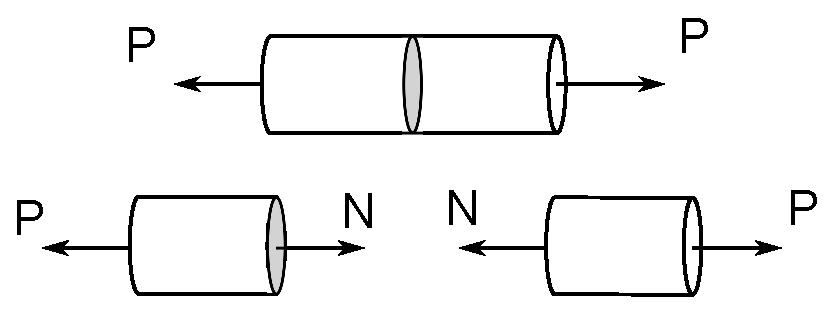
\includegraphics[width = 0.5\textwidth]{./Images/cylinder_forces.eps}
	\caption{Illustration av en stång som utsätts för en dragkraft och de orsakade inre krafterna.}
	\label{fig:cylinder_forces}
\end{figure}

Kraften $P$ i änderna propageras som inre krafter i stången. Om vi betraktar det indikerade tvärsnittet, manifesteras den inre kraften som en normalkraft på varje halva. Om vi definierar positiv riktning för normalkraften och dragkraften som i figuren, ger kraftjämvikten att $N = P$.

Om dragkraften blir en tryckkraft, ändrar givetvis normalkraften riktning. Detta kommer inte nödvändigtvis fram av kraftjämvikten. Därför väljer vi konventionen att normalkrafter alltid pekar ut från ytan. Då skulle kraftjämvikten för en pålagd tryckkraft bli $P = -N$, och vi ser att dragkrafter ger positiva normalkrafter och tryckkrafter negativa.

\paragraph{Statiskt bestämta och obestämta problem}
Ett problemt är statiskt bestämt om alla inre krafter och reaktionskrafter kan bestämmas enbart med jämvikt. Detta är möjligt om det verkar maximalt $3$ krafter i planet eller $6$ i rymden.

Om ett problem ej är statiskt bestämt, är det statiskt obestämt. Då räcker icke jämviktsekvationerna, och det motsvarar (ofta) att man kan ta bort ett element och vara kvar i jämvikt. För att lösa statiskt obestämda problem behövs typiskt materialsamband från hållfasthetsläran.

\paragraph{Spänning}
I hållfasthetslära är vi intresserade av påkänningen på materialet. Den beror av beloppet av normalkraften, men kan även spridas ut över tvärsnittet. Därför definierar vi spänningen
\begin{align*}
	\sigma = \frac{N}{A}.
\end{align*}
Jämvikten från innan ger
\begin{align*}
	\sigma = \frac{P}{A}.
\end{align*}

\paragraph{Deformation}
När en stång utsätts för spänning, kommer den att deformeras. Eftersom förlängningen av varje del kommer från kraftjämvikten mellan normalkraften och dragkraften, kommer förlängningen för en given dragkraft bero av längden. Vi definierar därför töjningen
\begin{align*}
	\varepsilon	= \frac{\delta}{L_{0}}
\end{align*}
där $L_{0}$ är stångens ursprungliga längd och $\delta$ är förlängningen.

\paragraph{Typer av samband i hållfasthetslära}
I hållfasthetsläran har vi tre typer av samband:
\begin{itemize}
	\item samband mellan krafter.
	\item samband mellan deformationer.
	\item konstitutiva samband (beskrivar materialbeteende).
\end{itemize}

\paragraph{Hookes lag}
Om man gör dragningsprov på olika material för små deformationer, blir plottet av $\sigma$ mot $\varepsilon$ approximativt linjär. Från detta får vi Hookes lag:
\begin{align*}
	\sigma = E\varepsilon.
\end{align*}
$E$ är elasticitetsmodulen, och beskrivar hur styvt materialet är. Hookes lag är ett exempel på ett konstitutivt samband.

Kombinationen av det vi har tills nu ger
\begin{align*}
	P = \frac{EA}{L}\delta
\end{align*}
för en homogen stång som utsätts för en dragkraft $P$.

Om ett material komprimeras, visar det sig att det elastiska beteendet ofta är likt, med samma elasticitetsmodul.

\paragraph{Normalspänning}
Vi utvidgar våran definition av spänning till spänningar som fördelas inhomogent över tvärsnittet vid att betrakta en inre kraft $\Delta F$ som verkar på ett arealement $\Delta A$, med riktningar som tidigare. Då definieras normalspänningen som
\begin{align*}
	\sigma = \lim\limits_{\Delta A\to 0}\frac{\Delta F}{\Delta A}.
\end{align*}

\paragraph{Normaltöjning}
Vi utvidgar även definitionen av töjning till töjningar som fördelas ojämnt över stavens längd. Om deformationen i en punkt är $u(x)$, ges töjningen av ett litet element med längd $\Delta x$ av
\begin{align*}
	\varepsilon = \lim\limits_{\Delta x\to 0}\frac{u(x + \Delta x) - u(x)}{\Delta x} = \dv{u}{x}.
\end{align*}
Vi ser av detta att töjningen är linjär, så vi kan addera bidrag till den.

\paragraph{Termoelasticitet}
Låt $T$ beteckna en stångs temperatur. En temperaturändring orsakar en termisk töjning
\begin{align*}
	\varepsilon_{T} = \alpha\Delta T,
\end{align*}
där $\alpha$ är längdutvidgningskoefficienten. Man behöver givetvis utgå från en referenstemperatur.

\paragraph{Allmänt enaxligt tillstånd}
Från det vi har sett hittils, kan vi skriva upp en differentialekvation som beskriver tillståndet i en stång.

Betrakta en stång med variabel tvärsnittsyta där det överallt i kroppen verkar en volymskraft $K(x)$ (kraft per volym), samt krafter $P_{\text{V}}$ respektiva $P_{\text{H}}$ i varje ända. Vi betraktar ett litet element med tjocklek $\dd{x}$. I ena ändan verkar kraften $K(x)A\dd{x}$ och en normalkraft $N(x + \dd{x})$ på grund av krafterna på volymelementet till höger, och i andra ändan verkar en normalkraft $N(x)$ på grund av krafterna på volyemelementet till vänster.

Kraftjämvikten ger
\begin{align*}
	N(x + \dd{x}) - N(x) + K(x)A\dd{x} &= 0, \\
	\dd{N}(x) + K(x)                   &= 0.
\end{align*}
Vi inför nu definitionen av töjning och skriver den som en linjärkombination av bidrag från spänning och termoelasticitet, vilket ger
\begin{align*}
	\varepsilon = \frac{\sigma}{E} + \alpha\Delta T, \\
	\sigma = E(\varepsilon - \alpha\Delta T).
\end{align*}
Kombinerad med definitionen av töjning ger det
\begin{align*}
	\dv{x} (\sigma A) + K(x)A &= 0, \\
	\dv{x} (EA(\varepsilon - \alpha\Delta T)) + K(x)A &= 0, \\
	\dv{x}\left(EA\dv{u}{x}\right) + K(x)A &= \dv{x}(EA\alpha\Delta T).
\end{align*}
Detta kommer med randvillkor, och är typiskt randvillkor i deformationen eller i spänningen. Eftersom spänningen är proportionell mot derivatan av deformationen, motsvarar dessa Dirichlet- respektiva Neumannvillkor.

\paragraph{Tvärkontraktion}
När man gör ett dragningsprov på en kropp, genomgår den deformation i längdriktning samtidigt som tjockleken minskar. Detta kallas tvärkontraktion. Töjningen $\varepsilon_{t}$ av tjockleken är relaterad till töjningen i längdriktning genom
\begin{align*}
	\varepsilon_{t} = -\nu\varepsilon,
\end{align*}
där $\nu$ är Poissons konstant. Termodynamiken ger att $-1\leq\nu\leq 0.5$.

\paragraph{Skjuvspänning}
Betrakta två plattor som ligger på varandra och dras åt motsatta håll av en kraft $F$ på varje. Om de inte dras isär, balanseras dragkrafterna av krafter i kontaktytan. Låt $A$ vara kontaktytan mellan plattorna. Då definieras skjuvspänningen som
\begin{align*}
	\tau = \frac{F}{A}.
\end{align*}

\paragraph{Deformation från skjuvkrafter}
Betrakta ett rätblock med basarea $A$ och höjd $H$ som dras av motsatt riktade krafter med belopp $F$ på varje sida, illustrerad i figur \ref{fig:rectangle_twist}.
\begin{figure}[!ht]
	\centering
	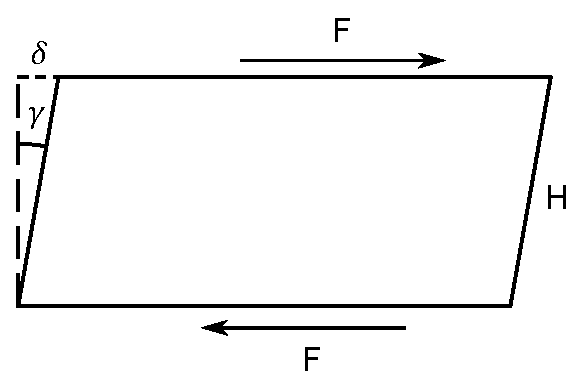
\includegraphics[width = 0.5\textwidth]{./Images/rectangle_twist.eps}
	\label{fig:rectangle_twist}
\end{figure}

Vi kan här definiera skjuvspänningen som
\begin{align*}
	\tau = \frac{F}{A},
\end{align*}
då vi kan tänka oss att plattorna som dras isär är tunna skikt i materialet. Skjuvkrafterna kommer skapa en deformation $\delta$ på en sida motsvarande vridning med en vinkel $\gamma$. Denna vinkeln uppfyller
\begin{align*}
	\tan{\gamma} = \frac{\delta}{H}.
\end{align*}
För små deformationer kan vi approximera
\begin{align*}
	\gamma = \frac{\delta}{H}.
\end{align*}
Experimentellt har man sett att
\begin{align*}
	\tau = G\gamma,
\end{align*}
där $G$ är skjuvmodulen.

\paragraph{Samband mellan materialstorheter}
För ett isotropt material gäller att
\begin{align*}
	G = \frac{E}{2(1 + \nu)}.
\end{align*}

\paragraph{Spänning i tre dimensioner}
Vi definierar spänningsvektorn
\begin{align*}
	\vb{s} = \lim\limits_{A \to 0}\frac{\vb{F}}{A}
\end{align*}
där $\vb{F}$ är kraften på ett litet arealement. Den har en komponent normalt på ytan, som är normalspänningen, och en komponent som är parallel med ytan, som är skjuvspänningen. Vi får
\begin{align*}
	\sigma = \vb{s}\cdot\vb{n},\ \tau^{2} = \abs{\vb{s}}^{2} - \sigma^{2}.
\end{align*}

\paragraph{Skjuvspänningar i tre dimensioner}
Snitta nu ut en infinitesimal kub från en godtycklig kropp. På ytorna, till exempel ytan som är normal på $x$-axeln, kan man dekomponera spänningsvektorn i en normalspänning $\sigma_{x}$ och två skjuvspänningar $\tau_{xy},\ \tau_{xz}$ (jag tänker på indexen som ``verkar på index 1 i riktning index 2''), och motsvarande för de andra sidorna. Om vi tittar på momentjämvikt kring kubens centrum i $x$-riktning och behandlar spänningen som oändrad genom kuben, fås
\begin{align*}
	2\tau_{yz}\dd{x}\dd{z}\cdot\frac{1}{2}\dd{y} - 2\tau_{zy}\dd{x}\dd{y}\cdot\frac{1}{2}\dd{z}        &= 0, \\
	\tau_{yz} &= \tau_{zy}.
\end{align*}
Faktorn $2$ tillkommer av att kraftjämvikt för kuben implicerar att skjuvspänningarna måste balanseras av en lika stor och motsatt riktad spänning på andra sidan. En motsvarande härledning kan göras för de andra sidorna.

\paragraph{Spänningsmatris}
Vi kan nu definiera en spänningsmatris
\begin{align*}
	S =
	\mqty[
		\sigma_{x} & \tau_{yx}  & \tau_{zx} \\
		\tau_{xy}  & \sigma_{y} & \tau_{zy} \\
		\tau_{xz}  & \tau_{yz}  & \sigma_{z}
	].
\end{align*}
Enligt argumentet ovan är denna symmetrisk.

\paragraph{Spänningar på godtycklig yta}
Om man har en godtycklig yta med normalvektor $\vb{n}$, kan det visas att spänningarna på ytan ges av
\begin{align*}
	\vb{s} = S\vb{n}.
\end{align*}
Vi kan då skriva
\begin{align*}
	\sigma &= \vb{n}^{T}S\vb{n}, \\
	\tau   &= \abs{S\vb{n}}^{2} - (\vb{n}^{T}S\vb{n})^{2}.
\end{align*}

\paragraph{Huvudspänningar}
Finns det orienteringar sådana att $\vb{s} = \sigma\vb{n}$? Att hitta sådana är ett egenvärdesproblem. Matematiken ger att det finns sådana orienteringar, och att de är ortogonala mot varandra.

Beteckna även den största respektiva minsta huvudspänningen som $\sigma_{1}$ respektiva $\sigma_{3}$. Då ges den maximala skjuvspänningen i materialet av
\begin{align*}
	\tau_{\text{max}} = \frac{\sigma_{1} - \sigma_{3}}{2}.
\end{align*}

\paragraph{Plana tillstånd}
Ett specialfall är när $z$-riktningen är en huvudriktning för spänningen. Då är skjuvspänningarna i $xy$-planet, dvs. $\tau_{zx} = \tau_{zy} = 0$. Om $\sigma_{z} = 0$, har man plan spänning.

Betrakta plan spänning på ett plan som bildar en vinkel $\phi$ med $y$-axeln. Normalvektorn ges av
\begin{align*}
	\vb{n} = \cos{\phi}\vb{e}_{x} + \sin{\phi}\vb{e}_{y}.
\end{align*}
Vi får då
\begin{align*}
	\sigma &= \sigma_{x}\cos^{2}{\phi} + \sigma_{y}\sin^{2}{\phi} + 2\tau_{xy}\sin{\phi}\cos{\phi}, \\
	\tau   &= \tau_{xy}\cos{2\phi} + \frac{\sigma_{y} - \sigma_{x}}{2}\sin{2\phi}.
\end{align*}

\paragraph{Mohrs spänningscirkel}
Mohrs spänningscirkel är ett sätt att grafiskt ta fram plana spänningar vid rotation av ett plan. För att konstruera cirkeln, rita upp ett $\sigma, \tau$-koordinatsystem och två punkter $(\sigma_{x}, \tau_{x, y})$ och $(\sigma_{y}, -\tau_{x, y})$, där dessa tas från något givet tillstånd. Dessa punkter skall vara i motstående änder av cirkeln, och från detta kan cirkeln ritas, som i figur \ref{fig:mohr_stress_circle}.

\begin{figure}[!ht]
	\centering
	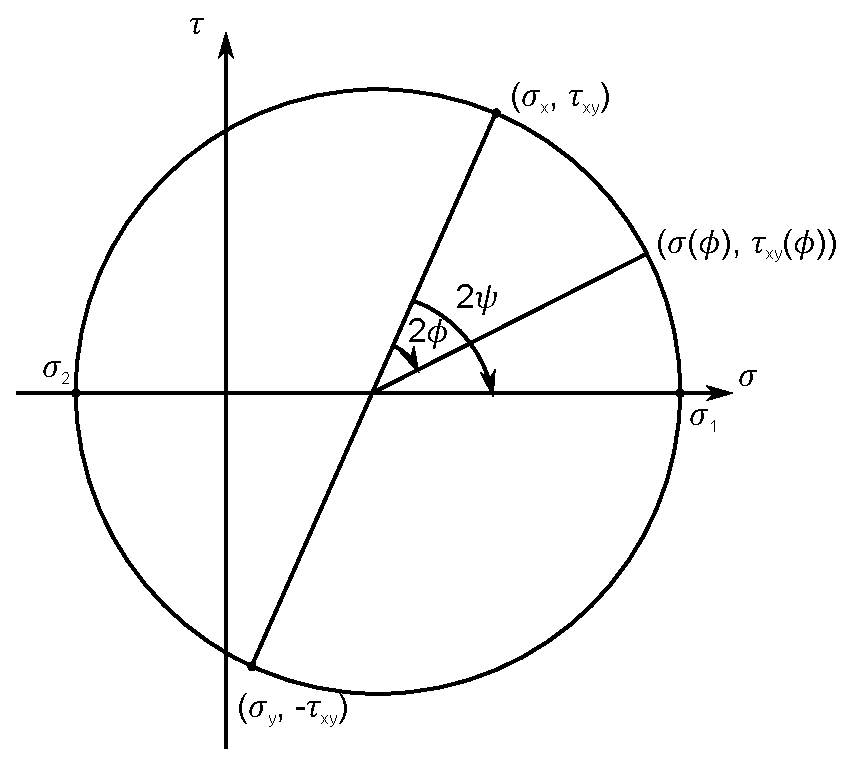
\includegraphics[width = 0.5\textwidth]{./Images/mohr_stress_circle.eps}
	\caption{Mohrs spänningscirkel.}
	\label{fig:mohr_stress_circle}
\end{figure}

En rotation moturs av koordinatsystemet med en vinkel $\phi$ motsvarar en rotation medurs av tillståndet på cirkeln med en vinkel $2\phi$.

Det visar sig att cirkeln skär $\sigma$-axeln i största och minsta huvudspänningen. Det finns även en vinkel $\psi$ som koordinatsystemet måste roteras med så att det blir parallellt med huvudriktningarna. Ur denna geometrin kan vi få följande samband, som är helt konsekventa med tensorbetraktningen gjort ovan:
\begin{align*}
	\sigma_{1}        &= \frac{\sigma_{x} + \sigma_{y}}{2} + \sqrt{\left(\frac{\sigma_{x} - \sigma_{y}}{2}\right)^{2} + \tau_{xy}^{2}}, \\
	\sigma_{2}        &= \frac{\sigma_{x} + \sigma_{y}}{2} - \sqrt{\left(\frac{\sigma_{x} - \sigma_{y}}{2}\right)^{2} + \tau_{xy}^{2}}, \\
	\tan(2\psi)       &= \frac{2\tau_{xy}}{\sigma_{x} - \sigma_{y}}, \\
	\tau_{\text{max}} &= \frac{\sigma_{1} - \sigma_{3}}{2}.
\end{align*}

\paragraph{Jämvikt i tre dimensioner}
Snitta ut en liten kub. Jämvikt i $x$-riktning ger
\begin{align*}
	\sigma(\vb{x} + \dd{x}\vb{e}_{x})\dd{y}\dd{z} - \sigma(\vb{x})\dd{y}\dd{z} + \tau_{zx}(\vb{x} + \dd{z}\vb{e}_{z})\dd{x}\dd{y} - \tau_{zx}(\vb{x})\dd{x}\dd{y} + \tau_{yx}(\vb{x} + \dd{y}\vb{e}_{y})\dd{x}\dd{z} - \tau_{yx}(\vb{x})\dd{x}\dd{z} = 0,
\end{align*}
vilket implicerar
\begin{align*}
	\del{x}{\sigma_{x}} + \del{y}{\tau_{xy}} + \del{z}{\tau_{zx}} = 0.
\end{align*}
På motsvarande sätt fås
\begin{align*}
	\del{x}{\tau_{xy}} + \del{y}{\sigma_{y}} + \del{z}{\tau_{yz}} &= 0, \\
	\del{y}{\tau_{xz}} + \del{y}{\tau_{yz}} + \del{z}{\sigma_{z}} &= 0.
\end{align*}
Om det finns volymkrafter i kroppen, dyker den även upp som en term här.

\paragraph{Töjning i tre dimensioner}
I tre dimensioner definieras töjningen i termer av båglängden som
\begin{align*}
	\varepsilon = \frac{\dd{s} - \dd{s_{0}}}{\dd{s_{0}}},
\end{align*}
där $\dd{s_{0}}$ är den odeformerade båglängden och $\dd{s}$ är den deformerade båglängden.

\paragraph{Tredimensionellt samband mellan töjning och deformation}
Betrakta en kropp som deformeras med en deformationsvektor $\vb{u}$. Snitta ut en kub och titta på två hörn i positioner $x$ och $x + \dv{x}$, med övriga koordinater lika. I det odeformerade läget är avståndet mellan dessa $\dd{s_{0}} = \dd{x}$. I det deformerade läget är avståndet
\begin{align*}
	\dd{s} &= (x + \dd{x} + u_{x}(x + \dd{x}, y, z)) - (x + u_{x}(x, y, z)) \\
	       &= \dd{x} + u_{x}(x + \dd{x}, y, z) - u_{x}(x, y, z) \\
	       &= \dd{x} + \del{x}{u_{x}}\dd{x},
\end{align*}
och töjningen i $x$-riktning ges av
\begin{align*}
	\varepsilon_{x} = \del{x}{u_{x}}.
\end{align*}
På samma sätt fås
\begin{align*}
	\varepsilon_{y} = \del{y}{u_{y}},\ \varepsilon_{z} = \del{z}{u_{z}}.
\end{align*}

\paragraph{Skjuvdeformation i tre dimensioner}
Betrakta en kub som deformeras i $xy$-planet. Sidan närmast $x$-axeln bildar vinkeln $\beta$ med $x$-axeln och sidan närmast $y$-axeln bildar vinkeln $\alpha$ med $y$-axeln. Den totala skjuvvinkeln ges av $\gamma_{yx} = \alpha + \beta$. Geometrin ger
\begin{align*}
	\gamma_{xy} = \frac{u_{x}(x, y + \dd{y}, z) - u_{x}(x, y, z)}{\dd{y}} + \frac{u_{y}(x + dd{x}, y, z) - u_{x}(x, y, z)}{\dd{x}} = \del{y}{u_{x}} + \del{x}{u_{y}}.
\end{align*}
på motsvarande sätt fås
\begin{align*}
	\gamma_{yz} = \del{z}{u_{y}} + \del{y}{u_{z}}, \gamma_{xz} = \del{z}{u_{x}} + \del{x}{u_{z}}.
\end{align*}

\paragraph{Töjningsmatrisen}
Vi definierar töjningsmatrisen
\begin{align*}
	T =
	\mqty[
		\varepsilon_{x}  & \varepsilon_{yx} & \varepsilon_{zx} \\
		\varepsilon_{xy} & \varepsilon_{y}  & \varepsilon_{zy} \\
		\varepsilon_{xz} & \varepsilon_{yz} & \varepsilon_{z}
	],
\end{align*}
där vi inför $\varepsilon_{xy} = \varepsilon_{yx} = \frac{1}{2}\gamma_{xy}$. Detta medför att $T$ är symmetrisk. Det gäller att töjningen i riktningen $\vb{n}$ ges av
\begin{align*}
	\varepsilon_{\vb{n}} = \vb{n}^{T}T\vb{n}.
\end{align*}

\paragraph{Huvudtöjningar}
Finns det orienteringar sådana att $T\vb{n} = \varepsilon\vb{n}$? Att hitta sådana är ett egenvärdesproblem. Matematiken ger att det finns sådana orienteringar, och att de är ortogonala mot varandra.

Beteckna även den största respektiva näst största huvudtöjningen som $\varepsilon_{1}$ respektiva $\varepsilon_{2}$. Då ges den maximala skjuvvinkeln i materialet av
\begin{align*}
	\gamma_{\text{max}} = \varepsilon_{1} - \varepsilon_{2}.
\end{align*}

\paragraph{Mohrs töjningscirkel}
Mohrs töjningscirkel är ett sätt att grafiskt ta fram plana töjningar vid rotation av ett plan. För att konstruera cirkeln, rita upp ett $\varepsilon, \frac{\gamma}{2}$-koordinatsystem och två punkter $(\varepsilon_{x}, \frac{\gamma_{x, y}}{2})$ och $(\varepsilon_{y}, -\frac{\gamma_{x, y}}{2})$, där dessa tas från något givet tillstånd. Dessa punkter skall vara i motstående änder av cirkeln, och från detta kan cirkeln ritas, som i figur \ref{fig:mohr_strain_circle}.

\begin{figure}[!ht]
	\centering
	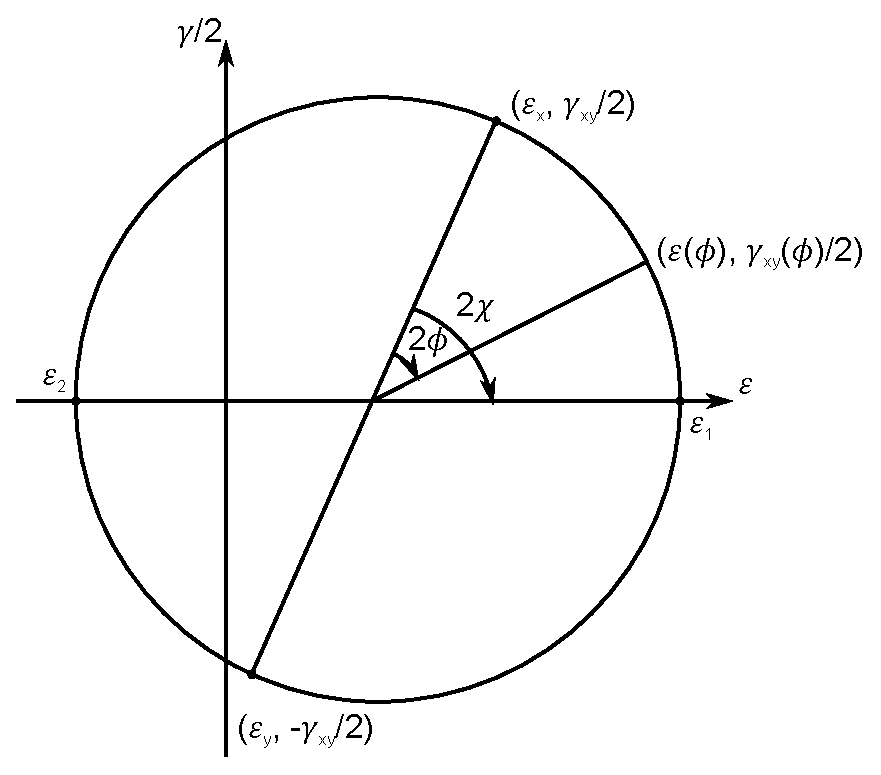
\includegraphics[width = 0.5\textwidth]{./Images/mohr_strain_circle.eps}
	\caption{Mohrs töjningscirkel.}
	\label{fig:mohr_strain_circle}
\end{figure}

En rotation moturs av planet med en vinkel $\phi$ motsvarar en rotation medurs av tillståndet på cirkeln med en vinkel $2\phi$.

Det visar sig att cirkeln skär $\varepsilon$-axeln i största och näst största huvudtöjningen. Det finns även en vinkel $\chi$ som koordinatsystemet måste roteras med så att det blir parallellt med huvudriktningarna. Ur denna geometrin kan vi få följande samband, som är helt konsekventa med tensorbetraktningen gjort ovan:
\begin{align*}
	\varepsilon_{1}     &= \frac{\varepsilon_{x} + \varepsilon_{y}}{2} + \sqrt{\left(\frac{\varepsilon_{x} - \varepsilon_{y}}{2}\right)^{2} + \left(\frac{\gamma_{xy}}{2}\right)^{2}}, \\
	\varepsilon_{2}     &= \frac{\varepsilon_{x} + \varepsilon_{y}}{2} - \sqrt{\left(\frac{\varepsilon_{x} - \varepsilon_{y}}{2}\right)^{2} + \left(\frac{\gamma_{xy}}{2}\right)^{2}}, \\
	\tan(2\psi)         &= \frac{\gamma_{xy}}{\varepsilon_{x} - \varepsilon_{y}}, \\
	\gamma_{\text{max}} &= \varepsilon_{1} - \varepsilon_{2}.
\end{align*}

\paragraph{Kompatibilitet i tre dimensioner}
Från definitionerna av elementerna i töjningsmatrisen kan man se att det gäller att
\begin{align*}
	2\del{x}{\del{y}{\varepsilon_{xy}}} &= \del[2]{y}{\varepsilon_{x}} + \del[2]{x}{\varepsilon_{y}}, \\
	2\del{y}{\del{z}{\varepsilon_{yz}}} &= \del[2]{z}{\varepsilon_{y}} + \del[2]{y}{\varepsilon_{z}}, \\
	2\del{z}{\del{x}{\varepsilon_{zx}}} &= \del[2]{x}{\varepsilon_{z}} + \del[2]{z}{\varepsilon_{x}}.
\end{align*}
Alltså är inte de olika töjningarna oberoende.

\paragraph{Linjärelastiska material}
I linjärelastiska material gäller sambandet $S = CT$, där $C$ är en fjärde ordningens tensor. Detta kan alternativt skrivas som $T = C^{-1}S$.

\paragraph{Hookes lag för isotropa material}
I isotropa material är alla riktningar lika. I dessa materialer gäller Hookes lag
\begin{align*}
	\varepsilon_{x} &= \frac{1}{E}(\sigma_{x} - \nu(\sigma_{y} + \sigma_{z})) + \alpha\Delta T, \\
	\varepsilon_{y} &= \frac{1}{E}(\sigma_{y} - \nu(\sigma_{x} + \sigma_{z})) + \alpha\Delta T, \\
	\varepsilon_{z} &= \frac{1}{E}(\sigma_{z} - \nu(\sigma_{x} + \sigma_{y})) + \alpha\Delta T, \\
	\gamma_{xy}     &= \frac{1}{G}\tau_{xy}, \\
	\gamma_{yz}     &= \frac{1}{G}\tau_{yz}, \\
	\gamma_{xz}     &= \frac{1}{G}\tau_{xz},
\end{align*}
där $E$ är elasticitetsmodulen, $G$ är skjuvmodulen och $\nu$ är Poissons tal.

\paragraph{Samband mellan elasticitetsmodul och skjuvmodul}
Betrakta ett plant skjuvtillstånd med skjuvspänning $\tau_{xy}$ för ett isotropt material. Med Moores spänningscirkel fås huvudspänningarna $\sigma_{1} = \tau_{xy},\ \sigma_{2} = -\tau_{xy}$. Hookes lag ger
\begin{align*}
	\varepsilon_{1} = \frac{1 + \nu}{E}\tau_{xy},\ \varepsilon_{2} = -\frac{1 + \nu}{E}\tau_{xy}.
\end{align*}
Mohrs töjningscirkel ger vidare
\begin{align*}
	\frac{\gamma_{xy}}{2} = \varepsilon_{1} = \frac{1 + \nu}{E}\tau_{xy}.
\end{align*}
Jämförelse med Hookes lag ger
\begin{align*}
	G = \frac{1}{2(1 + \nu)}E,
\end{align*}
vilket vi känner från innan.

\paragraph{Tunnväggiga tryckkärl}
Betrakta ett cylindrikskt tryckkärl med innerradie $a$ och väggtjocklek $h$ med ett inre tryck $p$. Vi kommer studera detta i cylindriska koordinater.

Det finns spänningar $\sigma_{z}$ och $\sigma_{\phi}$ i tryckkärlet. Cylindersymmetrin ger att båda dessa är oberoende av $\phi$. Det återstår bara att använda jämvikter för att beräkna dem.

Snitta nu ut en halvcylindrisk del med längd $\Delta z$, detta för att ej behöva betrakta radiella spänningar. Kraftjämvikt på ytan vi snittar genom ger
\begin{align*}
	2a\Delta zp - 2h\Delta z\sigma_{\phi} &= 0, \\
	\sigma_{\phi}                         &= \frac{pa}{h}.
\end{align*}

Snitta nu normalt på $z$-axeln. Om vi försummar kraftbidrag från annat än trycket i kärlet, ger kraftjämvikten
\begin{align*}
	2\pi ah\sigma_{z} - \pi a^{2}p &= 0, \\
	\sigma_{z}                     &= \frac{pa}{2h}.
\end{align*}

Om man tittar i radiell riktning, har vi randvillkoret $\sigma_{r} = -p$ på inre delen av mantelytan. Detta värdet är mycket mindre än de två andra spänningarna, så för tunnväggiga kärl approximerar vi $\sigma_{r} = 0.$

Vi får även töjningar av detta trycket. Om vi får en radiell töjning $u_{r}$, får vi en töjning $2\pi u_{r}$ i $\phi$-riktning.

Man kan göra samma beräkningar för ett sfäriskt kärl, och får
\begin{align*}
	\sigma_{\theta} = \sigma_{\phi} = \frac{pa}{2h}, \sigma_{r} = 0.
\end{align*}
Töjningarna ges av
\begin{align*}
	u_{\theta} = u_{\phi} = 2\pi u_{r}.
\end{align*}

\paragraph{Tjockväggiga tryckkärl}
Betrakta återigen ett cylindriskt tryckkärl, denna gången med innerradie $a$ och ytterradie $b$.

Snitta återigen normalt på $z$-axeln. Detta ger
\begin{align*}
	\sigma_{z} = \frac{pa^{2}}{b^{2} - a^{2}}.
\end{align*}

Snitta nu ut en bit av kärlet med vinkelbrädd $\Delta\phi$, höjd $\Delta z$ och tjocklek $\Delta r$. Vi har spänningar på alla sidor. Geometrin ger att spänningarna i $\phi$-riktning bildar vinkeln $\frac{\Delta\phi}{2}$ med den radiella normalen. Jämvikt i radiell riktning ger då
\begin{align*}
	(r + \Delta r)\Delta\phi\Delta z\sigma_{r}(r + \Delta r) - r\Delta\phi\Delta z\sigma_{r}(r) - 2\frac{\Delta\phi}{2}\Delta z\Delta r\sigma_{\phi} = 0.
\end{align*}
Detta kan lösas för att ge
\begin{align*}
	\frac{(r + \Delta r)\sigma_{r}(r + \Delta r) - r\sigma_{r}(r)}{\Delta r} - \sigma_{\phi} = 0,
\end{align*}
vilket i gränsen ger
\begin{align*}
	\dv{r}(r\sigma_{r}) - \sigma_{\phi} = 0.
\end{align*}

Notera att det ligger bakom att vissa skjuvspänningar blir $0$ för dena sortens symmetri.

Betrakta vidare deformationen och töjningarna. Vi får i radiell riktning
\begin{align*}
	\varepsilon_{r} = \frac{\Delta r + u_{r}(r + \Delta r) - u_{r}(r) - \Delta r}{\Delta r} \to\dv{u_{r}}{r}
\end{align*}
och i vinkelriktning
\begin{align*}
	\varepsilon_{\phi} = \frac{(r + u_{r})\Delta\phi - r\Delta\phi}{r\Delta\phi} = \frac{u_{r}}{r}.
\end{align*}
Vi kan kombinera dessa ekvationerna med Hookes lag för att få
\begin{align*}
	\dv{r}(r^{3}\dv{\sigma_{r}}{r}) = 0.
\end{align*}
På inre randen har vi
\begin{align*}
	\sigma_{r}(a) = -p.
\end{align*}
Om vi har en yttre last $q$, har vi även randvillkoret
\begin{align*}
	\sigma_{r}(a) = -q.
\end{align*}
Detta kan kombineras till att ge
\begin{align*}
	\sigma_{r}    &= \frac{p - \left(\frac{b}{a}\right)^{2}q}{\left(\frac{b}{a}\right)^{2} - 1} - \frac{p - q}{\left(\frac{b}{a}\right)^{2} - 1}\frac{b^{2}}{r^{2}}, \\
	\sigma_{\phi} &= \frac{p - \left(\frac{b}{a}\right)^{2}q}{\left(\frac{b}{a}\right)^{2} + 1} - \frac{p - q}{\left(\frac{b}{a}\right)^{2} - 1}\frac{b^{2}}{r^{2}}.
\end{align*}